\FloatBarrier
\section{حسگری فشرده}\label{ch:literature-review|sec:compressed-sensing}


\subsection{معرفی \lr{CS-MRI}}\label{ch:literature-review|sec:compressed-sensing|subsec:csmri}

\cite{Lustig_2007}

\begin{figure}[t!]
	\centering
	\subfigure[]{
		\copyrightbox[b]{
			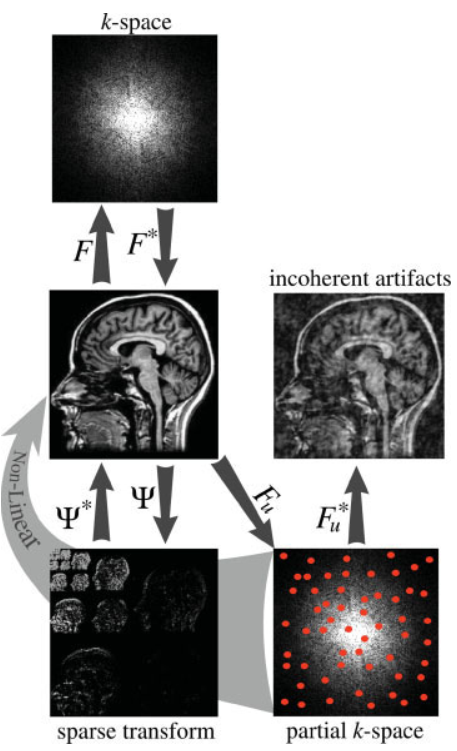
\includegraphics[width=0.4\linewidth]{chapters/chapter-3/figs/cs-mri-purpose}
			\label{fig:cs-mri-purpose}
	}{\doiSource{10.1002/mrm.21391}}}
	\hfill
	\subfigure[]{
		\copyrightbox[b]{
			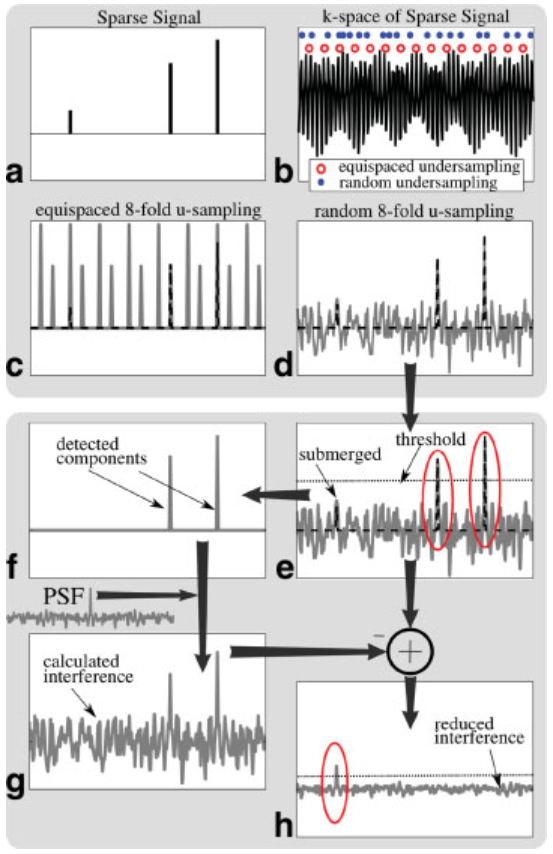
\includegraphics[width=0.4\linewidth]{chapters/chapter-3/figs/cs-mri-incoherency}
			\label{fig:cs-mri-incoherency}
	}{\doiSource{10.1002/mrm.21391}}}
	\caption{}
\end{figure}



\FloatBarrier
\subsection{معرفی روش \lr{ALOHA }}\label{ch:literature-review|sec:compressed-sensing|subsec:aloha}


ماتریس ساختاریافته هنکل
\LTRfootnote{Structured Hankel Matrix}
را می‌توان به شکل زیر تعریف کرد.

\removevspace
\begin{equation}\label{eq:HankelStructuredMatrix}
	\mathcal{H}(\mathbf{x})=
	\left[\begin{array}{cccc}
		x[0] & x[1] & \cdots & x[d-1] \\
		x[1] & x[2] & \cdots & x[d] \\
		\vdots & \vdots & \ddots & \vdots \\
		x[n-d] & x[n-d+1] & \cdots & x[n-1]
	\end{array}\right]
\end{equation}


